%===============================================================================
% LaTeX sjabloon voor de bachelorproef toegepaste informatica aan HOGENT
% Meer info op https://github.com/HoGentTIN/bachproef-latex-sjabloon
%===============================================================================

\documentclass{bachproef-tin}
\usepackage[backend=biber,style=apa]{biblatex}
\addbibresource{bachproef-tin.bib}
\usepackage{hogent-thesis-titlepage} % Titelpagina conform aan HOGENT huisstijl

%%---------- Documenteigenschappen ---------------------------------------------
% TODO: Vul dit aan met je eigen info:

% De titel van het rapport/bachelorproef
\title{Herkenning van schriftsystemen via een convolutioneel neuraal netwerk}

% Je eigen naam
\author{Vercleyen Vital}

% De naam van je promotor (lector van de opleiding)
\promotor{Steven Van Impe}

% De naam van je co-promotor. Als je promotor ook je opdrachtgever is en je
% dus ook inhoudelijk begeleidt (en enkel dan!), mag je dit leeg laten.
\copromotor{Glenn Vanlooveren}

% Indien je bachelorproef in opdracht van/in samenwerking met een bedrijf of
% externe organisatie geschreven is, geef je hier de naam. Zoniet laat je dit
% zoals het is.
\instelling{---}

% Academiejaar
\academiejaar{2018-2019}

% Examenperiode
%  - 1e semester = 1e examenperiode => 1
%  - 2e semester = 2e examenperiode => 2
%  - tweede zit  = 3e examenperiode => 3
\examenperiode{2}

%===============================================================================
% Inhoud document
%===============================================================================

\begin{document}

%---------- Taalselectie -------------------------------------------------------
% Als je je bachelorproef in het Engels schrijft, haal dan onderstaande regel
% uit commentaar. Let op: de tekst op de voorkaft blijft in het Nederlands, en
% dat is ook de bedoeling!

%\selectlanguage{english}

%---------- Titelblad ----------------------------------------------------------
\inserttitlepage

%---------- Samenvatting, voorwoord --------------------------------------------
\usechapterimagefalse
%%=============================================================================
%% Voorwoord
%%=============================================================================

\chapter*{\IfLanguageName{dutch}{Woord vooraf}{Preface}}
\label{ch:voorwoord}


Voor u ligt een onderzoek naar het herkennen van schriftsystemen door middel van deep learning.
Dit is geschreven in het kader van de afstudeerrichting Toegepaste Informatica aan de Hoge School Gent.
Van februari 2019 tot en met mei 2019 ben ik bezig geweest met het onderzoek en het schrijven van mijn bachelorproef.

Samen met mijn promotor, Steven Van Impe, heb ik de onderzoeksvraag voor deze bachelorproef bedacht.
Ik had veel baat aan de technische hulp die ik kreeg van Glenn Van Looveren, hij beantwoordde steeds mijn vragen waardoor ik steeds verder kon met mijn onderzoek.

Bij dezen wil ik graag mijn begeleiders bedanken voor de fijne begeleiding en hun ondersteuning tijdens dit traject. Ook wil ik alle respondenten bedanken die mee hebben gewerkt aan dit onderzoek. Zonder hun medewerking had ik dit onderzoek nooit kunnen voltooien.

Tevens wil ik ook mijn stagecollega Joris Opsommer bedanken die mij vaak heeft bijgestaan bij dit onderzoek.
Bovendien ben ik ook dankbaar voor de wijze raad van mijn vrienden en familie en met nadruk op mijn vriendin Aya Coppens die mij elke dag motivatie en inspiratie gaf.

Tot slot wil ik zeker mijn ouders bedanken die ervoor zorgden dat ik aan mijn studie kon beginnen en die zal afmaken.

Ik wens u veel leesplezier toe.

Vercleyen Vital
%% TODO:
%% Het voorwoord is het enige deel van de bachelorproef waar je vanuit je
%% eigen standpunt (``ik-vorm'') mag schrijven. Je kan hier bv. motiveren
%% waarom jij het onderwerp wil bespreken.
%% Vergeet ook niet te bedanken wie je geholpen/gesteund/... heeft


%%=============================================================================
%% Samenvatting
%%=============================================================================

% TODO: De "abstract" of samenvatting is een kernachtige (~ 1 blz. voor een
% thesis) synthese van het document.
%
% Deze aspecten moeten zeker aan bod komen:
% - Context: waarom is dit werk belangrijk?
% - Nood: waarom moest dit onderzocht worden?
% - Taak: wat heb je precies gedaan?
% - Object: wat staat in dit document geschreven?
% - Resultaat: wat was het resultaat?
% - Conclusie: wat is/zijn de belangrijkste conclusie(s)?
% - Perspectief: blijven er nog vragen open die in de toekomst nog kunnen
%    onderzocht worden? Wat is een mogelijk vervolg voor jouw onderzoek?
%
% LET OP! Een samenvatting is GEEN voorwoord!

%%---------- Nederlandse samenvatting -----------------------------------------
%
% TODO: Als je je bachelorproef in het Engels schrijft, moet je eerst een
% Nederlandse samenvatting invoegen. Haal daarvoor onderstaande code uit
% commentaar.
% Wie zijn bachelorproef in het Nederlands schrijft, kan dit negeren, de inhoud
% wordt niet in het document ingevoegd.

\IfLanguageName{english}{%
\selectlanguage{dutch}
\chapter*{Samenvatting}



\selectlanguage{english}
}{}

%%---------- Samenvatting -----------------------------------------------------
% De samenvatting in de hoofdtaal van het document

\chapter*{\IfLanguageName{dutch}{Samenvatting}{Abstract}}

Karakterherkenning is een veel besproken onderwerp binnen artificiële intelligentie, hierin gaat veel aandacht naar het herkennen van karakters in een specifiek schriftsysteem.
Wat dit onderzoek trachtte te bereiken is het maken van een convolutioneel neuraal netwerk dat verschillende schriftsystemen kan onderscheiden.
Dit kan een voordeel bieden aan letterkundigen die een opdracht krijgen binnenin de forensische letterkunde om een bepaald document met een ongekend schriftsysteem te herkennen en te lokaliseren.

Het onderscheiden van schriftsystemen met behulp van artificiële intelligentie is al onderzocht maar dit steeds op basis van woorden en paragrafen.
Dit onderzoek pakt het anders aan, het gebruikt een convolutioneel neuraal netwerk om schriftsystemen te herkennen op basis van een individueel karakter, dit bied een voordeel aangezien individuele karakters vaak voorkomen in documenten wanneer de grootste inhoud van het document geschreven is in een ander schriftsysteem.

De inhoud van dit onderzoek bestaat uit een stand van zaken waarin de gebruikte technologieën worden besproken samen met een bespreking van het de stand van zaken in dit onderzoek. \\
Vervolgens is een methodologie uitgeschreven waarin wordt uitgelegd hoe te werk is gegaan bij het verzamelen van data, het ontwerpen en trainen van het convolutioneel neuraal netwerk en een bespreking van de vooropgestelde experimenten. \\
Vervolgens is er een bespreking aanwezig van de uitgevoerde experimenten en worden de resultaten besproken en vergeleken met de verwachtingen. \\
Uiteindelijk is er een conclusie waarin een antwoord wordt gegeven op de onderzoeksvraag, er wordt besproken hoe dit onderzoek een meerwaarde bracht aan het vakgebied en een reflectie van de uitgevoerde experimenten.

%---------- Inhoudstafel -------------------------------------------------------
\pagestyle{empty} % Geen hoofding
\tableofcontents  % Voeg de inhoudstafel toe
\cleardoublepage  % Zorg dat volgende hoofstuk op een oneven pagina begint
\pagestyle{fancy} % Zet hoofding opnieuw aan

%---------- Lijst figuren, afkortingen, ... ------------------------------------

% Indien gewenst kan je hier een lijst van figuren/tabellen opgeven. Geef in
% dat geval je figuren/tabellen altijd een korte beschrijving:
%

%
% De korte beschrijving wordt gebruikt voor deze lijst, de uitgebreide staat bij
% de figuur of tabel zelf.

\listoffigures

 
\listoftables

% Als je een lijst van afkortingen of termen wil toevoegen, dan hoort die
% hier thuis. Gebruik bijvoorbeeld de ``glossaries'' package.
% https://www.overleaf.com/learn/latex/Glossaries

%---------- Kern ---------------------------------------------------------------

% De eerste hoofdstukken van een bachelorproef zijn meestal een inleiding op
% het onderwerp, literatuurstudie en verantwoording methodologie.
% Aarzel niet om een meer beschrijvende titel aan deze hoofstukken te geven of
% om bijvoorbeeld de inleiding en/of stand van zaken over meerdere hoofdstukken
% te verspreiden!

%%=============================================================================
%% Inleiding
%%=============================================================================

\chapter{\IfLanguageName{dutch}{Inleiding}{Introduction}}
\label{ch:inleiding}

%%De inleiding moet de lezer net genoeg informatie verschaffen om het onderwerp te begrijpen en in te zien waarom de onderzoeksvraag de moeite waard is om te onderzoeken. In de inleiding ga je literatuurverwijzingen beperken, zodat de tekst vlot leesbaar blijft. Je kan de inleiding verder onderverdelen in secties als dit de tekst verduidelijkt. Zaken die aan bod kunnen komen in de inleiding~\autocite{Pollefliet2011}:

%\begin{itemize}
  %%\item context, achtergrond
  %%\item afbakenen van het onderwerp
  %%\item verantwoording van het onderwerp, methodologie
  %%\item probleemstelling
  %%\item onderzoeksdoelstelling
  %%\item onderzoeksvraag
  %%\item \ldots
%%\end{itemize}

Naast het gesproken woord en de verschillen in talen hierin zijn er ook verschillende soorten schriftsystemen die gebruikt worden in deze talen.
Het onderscheiden van deze systemen is niet altijd vanzelfsprekend, vele van deze zijn vaak zeer verschillend maar een aantal zijn ook zeer gelijkaardig.
Het herkennen hiervan is altijd al een onderwerp geweest in deep learning, echter is er niet veel onderzoek uitgevoerd naar het onderscheiden van specifieke karakters door middel van een convolutional neural network. 
Bovendien is het belangrijk om te weten welk soort schrift er wordt gebruikt bij een meertalige omgeving die ook meerdere schriften bevat vooraleer een karakter herkenner kan gebruikt worden.

Het automatisch herkennen van schriftsystemen is zeer gewild bij letterkundigen aangezien er bij de forensische taalkunde waarbij er gevraagd wordt om een bepaald document geschreven in een onbekend schrift te lokaliseren. Heel vaak gaat het daarbij vaak om heel onbekende of geheime schriftsystemen, of gewoon gecodeerde taal. 

Ook is het classificeren van karakters uit verschillende schriftsystemen ook toepasselijk bij automatische transcriptie of het vinden van documenten op het internet die geschreven zijn in een specifiek schriftsysteem.

In dit onderzoek wordt er nagegaan of het mogelijk is om door middel van een convolutional neural network verschillende schriftsystemen te classificeren en zodanig het proces te versnellen voor letterkundigen die trachten een bepaald schriftsysteem te identificeren. 

 

\section{\IfLanguageName{dutch}{Probleemstelling}{Problem Statement}}
\label{sec:probleemstelling}


Het probleem dat wordt aangepakt en verder ook onderzocht wordt is vooral het helpen van deskundigen in de forensische letterkunde, deze krijgen af en toe een taak opgelegd om een bepaald schriftsysteem te herkennen en zodanig te lokaliseren.
Als het mogelijk is om met behulp van een convolutional neural network bepaalde software te ontwikkelen kunnen deze taalkundigen sneller hun taak volbrengen en dan ook de gekoppelde zaak versnellen.
Meer specifiek gaat het hier over Chris Bulcaen, de curriculum manager bij Taal & Letterkunde aan de Ugent.
Hij concludeerde dat dit inderdaad een meerwaarde zou geven in de forensische letterkunde en dat hierdoor het werk zeker versneld zou worden.

Ook zouden meerdere bedrijven die bezig zijn met karakterherkenning en vertaling hier baan aan hebben.
Deze zijn meer bezig met het herkennen van karakters in één schriftsysteem.
Wanneer er een systeem zou bestaan dat eerst en vooral het schriftsysteem zou herkennen kan dit voordelig zijn wanneer er achteraf dan de correcte karakterherkenning toepast voor het juiste schriftsysteem.


%Uit je probleemstelling moet duidelijk zijn dat je onderzoek een meerwaarde heeft voor een concrete doelgroep. De doelgroep moet goed gedefinieerd en afgelijnd zijn. Doelgroepen als ``bedrijven,'' ``KMO's,'' systeembeheerders, enz.~zijn nog te vaag. Als je een lijstje kan maken van de personen/organisaties die een meerwaarde zullen vinden in deze bachelorproef (dit is eigenlijk je steekproefkader), dan is dat een indicatie dat de doelgroep goed gedefinieerd is. Dit kan een enkel bedrijf zijn of zelfs één persoon (je co-promotor/opdrachtgever).

\section{\IfLanguageName{dutch}{Onderzoeksvraag}{Research question}}
\label{sec:onderzoeksvraag}


Is het mogelijk om onherkenbare handgeschreven geschriften door middel van een convolutional neural network te herkennen, het correcte schriftsysteem vast te stellen en zo het proces te versnellen voor letterkundigen.

%Wees zo concreet mogelijk bij het formuleren van je onderzoeksvraag. Een onderzoeksvraag is trouwens iets waar nog niemand op dit moment een antwoord heeft (voor zover je kan nagaan). Het opzoeken van bestaande informatie (bv. ``welke tools bestaan er voor deze toepassing?'') is dus geen onderzoeksvraag. Je kan de onderzoeksvraag verder specifiëren in deelvragen. Bv.~als je onderzoek gaat over performantiemetingen, dan 

\section{\IfLanguageName{dutch}{Onderzoeksdoelstelling}{Research objective}}
\label{sec:onderzoeksdoelstelling}

Het beoogde resultaat van deze bachelorproef is het ontwikkelen van een convolutional neural network waarbij er een aantal verschillende n schriftsystemen zo accuraat mogelijk van elkaar kunnen worden onderscheiden.
Een model waarbij alle soorten schriftsystemen herkend kunnen worden is niet het beoogde resultaat aangezien dit veel meer tijd zou kosten bij het verzamelen van data, dit wordt duidelijk in het onderzoek.

%Wat is het beoogde resultaat van je bachelorproef? Wat zijn de criteria voor succes? Beschrijf die zo concreet mogelijk. Gaat het bv. om een proof-of-concept, een prototype, een verslag met aanbevelingen, een vergelijkende studie, enz.

\section{\IfLanguageName{dutch}{Opzet van deze bachelorproef}{Structure of this bachelor thesis}}
\label{sec:opzet-bachelorproef}

% Het is gebruikelijk aan het einde van de inleiding een overzicht te
% geven van de opbouw van de rest van de tekst. Deze sectie bevat al een aanzet
% die je kan aanvullen/aanpassen in functie van je eigen tekst.

De rest van deze bachelorproef is als volgt opgebouwd:

In Hoofdstuk~\ref{ch:stand-van-zaken} wordt een overzicht gegeven van de stand van zaken binnen het onderzoeksdomein, op basis van een literatuurstudie.

In Hoofdstuk~\ref{ch:methodologie} wordt de methodologie toegelicht en worden de gebruikte onderzoekstechnieken besproken om een antwoord te kunnen formuleren op de onderzoeksvragen.

% TODO: Vul hier aan voor je eigen hoofstukken, één of twee zinnen per hoofdstuk

In Hoofdstuk~\ref{ch:conclusie}, tenslotte, wordt de conclusie gegeven en een antwoord geformuleerd op de onderzoeksvragen. Daarbij wordt ook een aanzet gegeven voor toekomstig onderzoek binnen dit domein.
\chapter{\IfLanguageName{dutch}{Stand van zaken}{State of the art}}
\label{ch:stand-van-zaken}

% Tip: Begin elk hoofdstuk met een paragraaf inleiding die beschrijft hoe
% dit hoofdstuk past binnen het geheel van de bachelorproef. Geef in het
% bijzonder aan wat de link is met het vorige en volgende hoofdstuk.

In dit hoofdstuk wordt de stand van zaken besproken.
Dit bevat wat er al onderzocht is over het onderwerp dat in deze bachelorproef besproken wordt.
De stand van zaken zorgt ervoor dat een lezer die niet op de hoogte is van het besproken onderwerp kan volgen met het lezen hiervan.

% Pas na deze inleidende paragraaf komt de eerste sectiehoofding.

%Dit hoofdstuk bevat je literatuurstudie. De inhoud gaat verder op de inleiding, maar zal het onderwerp van de bachelorproef *diepgaand* uitspitten. De bedoeling is dat de lezer na lezing van dit hoofdstuk helemaal op de hoogte is van de huidige stand van zaken (state-of-the-art) in het onderzoeksdomein. Iemand die niet vertrouwd is met het onderwerp, weet nu voldoende om de rest van het verhaal te kunnen volgen, zonder dat die er nog andere informatie moet over opzoeken \autocite{Pollefliet2011}.

%Je verwijst bij elke bewering die je doet, vakterm die je introduceert, enz. naar je bronnen. In \LaTeX{} kan dat met het commando \texttt{$\backslash${textcite\{\}}} of \texttt{$\backslash${autocite\{\}}}. Als argument van het commando geef je de ``sleutel'' van een ``record'' in een bibliografische databank in het Bib\LaTeX{}-formaat (een tekstbestand). Als je expliciet naar de auteur verwijst in de zin, gebruik je \texttt{$\backslash${}textcite\{\}}.
%Soms wil je de auteur niet expliciet vernoemen, dan gebruik je \texttt{$\backslash${}autocite\{\}}. In de volgende paragraaf een voorbeeld van elk.

%\textcite{Knuth1998} schreef een van de standaardwerken over sorteer- en zoekalgoritmen. Experten zijn het erover eens dat cloud computing een interessante opportuniteit vormen, zowel voor gebruikers als voor dienstverleners op vlak van informatietechnologie~\autocite{Creeger2009}.

\section{Schriftsystemen en hun groepen}

Onderzoek naar verschillende soorten schriftsystemen is simpel terug te vinden aangezien het beschouwd wordt als een echte wetenschap sinds de 20e eeuw.
Alhoewel het onderzoek vooral aanwezig was in de westerse wereld was er een soort van discriminatie aanwezig in dit vak.

Een van de eerste boeken over de verschillen in schriftsystemen was het boek genaamd 'A Study of Writing', geschreven door I. J. Gelb in 1952. \autocite{Gelb1952}
De schrijver trachtte een basis neer te leggen voor de ontwikkeling van een nieuwe wetenschap die de naam 'grammatologie' zou gekregen hebben.
Deze nieuwe wetenschap probeerde standaard principes vast te leggen over het gebruik en de evolutie van het schrift op een vergelijkende wijze.
Dit was anders dan de voorgaande studies in het vak van schriftsystemen aangezien het een aantal systemen vergeleek met andere en niet enkel keek naar de geschiedenis en evolutie van een systeem.
Dit boek bracht duidelijkheid in andere schriftsystemen dan dat de westerse bewoner gewoon was. 
In dit boek legde de schrijver uit hoe taalkundigen de gesproken taal zagen als iets dat meer biologisch is ontwikkeld en dit al doorheen de hele evolutie van de mens.
Daarentegen vermeldde hij dat schriftsystemen zijn ontwikkeld als een technologie en dit enkel in de voorbije duizenden jaren en duidelijk meer een culturele dan een biologische schenking zijn.

In de jaren 60 waren er nog grote misopvattingen aanwezig bij de taalkundigen.
Bijvoorbeeld beschouwde Jack Goody, een toenmalig taalkundige, het Chinese schrift als een gelimiteerd systeem aangezien hij vond dat het incapabel was om vele ideeën uit te drukken en de adoptie van westerse talen in deze cultuur hinderde.

Gelukkig is in de laatste jaren alles veranderd, de studie naar schriftsystemen is een gerespecteerde wetenschap in de taalkunde en is daarbij ook een beoefende wetenschap. 
Met dank aan de globalisatie is er een groter begrip gevormd voor andere talen dan die in de westerse wereld.
Aangezien het duidelijk is dat schriftsystemen ontwikkeld zijn uit de cultuur en niet uit de biologische geschiedenis is het interessanter om dit te bestuderen aangezien het nieuwer en flexibeler is.

Een schriftsysteem, technisch beschreven als een schrift of orthografie kan geclassificeerd worden onder verschillende groepen. \autocite{David} \autocite{Allan2015}
Er zijn een aantal soorten groepen en allen zijn simpel van elkaar te onderscheiden maar in dit onderzoek wordt er gefocust op de drie meest voorkomende.

Eén daarvan is het logografische schrift of anders verwoord, het beeldschrift.
Bij deze groep zijn volledige woorden uitgeschreven als een volledig teken dat compleet op zijn eigen staat en geen hulp nodig heeft van andere tekens om het te kunnen lezen.
Zoals hierboven reeds vermeld werd dit vroeger als een gelimiteerd schrift beschouwd aangezien het niet mogelijk is om andere talen uit te drukken in dit schrift.
Dit is niet correct aangezien alle logografische schriften nooit puur logografisch zijn. Bij deze schriften zijn er naast woord-gebaseerde tekens ook klank-gebaseerde tekens aanwezig voor het representeren van woorden die niet eigen zijn aan de taal of het schrift.
Het logografisch schrift wordt bekeken als een van de oudste groepen, de talen die onder deze groepen vallen zijn vaak ook oude schriften waardoor ze tijd hadden om zich volledig te ontwikkelen en zijn daardoor interessant in het heden.

Een andere groep is het syllabisch of lettergrepenschrift.
Bij deze schriften stellen de symbolen een klinker of een combinatie van medeklinkers en klinkers voor, simpeler gezegd stelt elk symbool simpelweg een lettergreep voor.
Lettergrepenschriften zijn vaak schriften die vroeger vooral werden gebruikt, in onze tijd komen deze schriften zelden voor.
een lettergrepenschrift komt deze tijd meer voor bij een logografisch schrift, dit zijn de klank-gebaseerde tekens zoals hierboven vermeld.

Onder het syllabsich schrift valt een andere groep die nog vaak voorkomt en niet mag weggelaten worden.
Deze groep is gekend als een consonantenschrift, deze schriften bestaan enkel uit medeklinkers waarbij de klinkers compleet worden genegeerd, hierdoor komt er bij het uitspreken van deze schriften wat gokken bij te pas en ervaring om de juiste klank te vinden.


De laatste en grootste groep is een groep die vooral voorkomt in de westerse wereld en momenteel ook de meest gebruikte, het alfabetisch schrift.
De reden waarom dit de meest voorkomende groep is is omdat het een van de simpelste groepen is in vergelijking met de andere.
Het alfabetisch schrift representeert de fonologische structuur van de gesproken taal die dit schrift gebruikt, de geschreven taal representeert de uitgesproken klank.

Hier zijn verschillen aanwezig in de klank tussen de talen die dit schrift gebruiken, De Engelse uitspraak voor het woord 'hand' is bijvoorbeeld verschillend tegenover de Nederlandse uitspraak van dit zelfde woord.
Deze verschillen komen voort uit het uitspreken van dit schrift, vaak zijn ze te vinden in hoe de lippen, tong, gehemelte en keel wordt gebruikt. Bij alle uitgesproken talen worden deze verschillend gebruikt en vormen daardoor steeds een andere soort klank. 

Het alfabetisch schrift is er een die de andere schriften overtreft aangezien het fonologisch is, hiermee kunnen een groot deel van de reeds bestaande klanken worden uitgedrukt.
Een voorbeeld hiervan is het universele fonologische schrift dat bestaat uit een aantal symbolen die weergeven hoe een bepaald woord moet worden uitgesproken.
De klanken worden dan letterlijk uitgeschreven op papier en dit enkel op basis van gehoor.


\autocite{Rickandie2016} Het schrift is in de eerste vorm uitgevonden door Semitische volkeren met als bekendste de Feniciërs. Het alfabetisch schrift werd door veelvuldige contacten met omringende volken overgenomen door de Grieken, Hebreeërs en Arabieren. Via de Grieken namen ook de Romeinen het over. Gaandeweg hebben er echter veel aanpassingen plaatsgevonden tot het uiteindelijke eenvoudige schrift. De naam van het schrift is afgeleid van het Griekse alpha en bèta dat de eerste twee symbolen zijn van het Griekse alfabet.


\section{Artificiële intelligentie}

Aangezien het programma dat zal worden geschreven een aantal beslissingen moet maken en kunnen nadenken over deze beslissingen wijst dit automatisch op een technologische term, namelijk artificiële intelligentie.
Het mogelijk maken voor programma's om te denken, doen en leren als een mens.
Of een meer genuanceerde definitie.

Artificiële of kunstmatige intelligentie is een interdisciplinair concept dat de mogelijkheid bestudeert voor het ontwikkelen van machines capabel om interactie aan te gaan met hun omgeving en in te werken op de ontvangen data op een manier die als intelligent beschouwd kan worden.

De term artificiële intelligentie werd als eerst gebruikt door John McCarthy in 1956, een Stanford onderzoeker.
Hij bedacht de term en legde AI vast als een branche van de computerwetenschap.

Artificiële intelligentie is in onze tijd al redelijk ontwikkeld en blijft maar groeien, het is tegenwoordig overal te vinden in het leven van de doodgewone mens.
Een eenvoudig voorbeeld hiervan is Siri of Alexa, een persoonlijke assistent. Deze en anderen zijn al in staat om onze stem te herkennen, de toegankelijke informatie te analyseren en een zo compleet mogelijk antwoord terug te geven. Deze assistenten leren voortdurend meer over hun gebruiker waardoor ze beter en gemakkelijker kunnen voldoen aan de persoonlijke eisen van de gebruiker.

Experten voorspellen dat artificiële intelligentie binnen het volgende decennia de mens zal overtreffen in het vervolledigen van simpele opdrachten zoals het vertalen van buitenlandse talen, het schrijven van verslagen of het besturen van een wagen. Maar het kunnen schrijven van een hooggewaardeerd boek of de taken overnemen van een chirurg zou nog wat langer kunnen duren. \autocite{Katja2018}



\section{Machine learning en deep learning}

Terwijl artificiële intelligentie, machine learning en deep learning vaak door elkaar worden gebruikt zijn er een aantal verschillen die deze drie termen van elkaar onderscheiden. Een manier om de relatie tussen deze te visualiseren is door middel van concentrische cirkels.
Artificiële intelligentie is hierbij de overkoepelende cirkel en dan ook de buitenste laag die het gehele domein van de studie voorstelt. machine learning is dan een cirkel binnen in artificiële intelligentie. Als laatste heb je deep learning, de kleinste cirkel, dat een verfijning is van machine learning en de meeste artificiële intelligentie applicaties die vandaag worden gebruikt, representeert. (Figuur \ref{tab:cirkels})

\begin{figure}
    \centering
    
    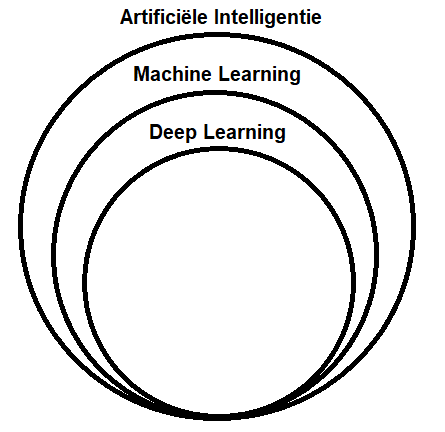
\includegraphics[scale=0.6]{img/cirkels.png}
    \caption{Voorstelling van de concentrische cirkels}
    \label{tab:cirkels}
\end{figure}

machine learning is simpel uitgelegd het proces van het ontwikkelen van machines die in staat zijn datasets op te halen, algoritmes uit te voeren op deze data en vervolgens zichzelf te trainen en uiteindelijk waardevolle inzichten te ontwikkelen gebaseerd op deze datasets.
Het grootste verschil tussen machine learning en artificiële intelligentie is dat machine learning niet expliciet afhangt van de geschreven code van zijn ontwikkelaar. machine learning gebruikt eerder geschreven code als een startpunt en halen daarna data en informatie op waarop gestudeerd wordt, veel gelijkend op hoe een student zou studeren voor een examen.

\autocite{Arthur Samuel, 1959} "The ability to learn without being explicitly programmed."

De term machine learning werd voor het eerst gebruikt in 1959 door Arthur Samuel. In de jaren 80 daarentegen kreeg het vak meer aandacht en werd er meer onderzoek in gestoken waardoor een grote groei plaatsvond die nog altijd even sterk is in het heden. \autocite{KeithD.2019} 
Momenteel wordt machine learning vooral gebruikt bij het herkennen van gezichten, stemcommando's en het vertalen van talen. Vooral terug te vinden bij persoonlijke assistenten zoals Siri of Alexa, zoals hierboven vermeld.

Een voorbeeld van machine learning is het voorspellen van de prijs van een wagen.
De enigste taak die machine learning moet volbrengen is het geven van een best passend antwoord maar met invloed van vele parameters, een model dat de prijs zou kunnen voorspellen van een wagen gaat als volgt.
Eerst en vooral kijkt het model naar een hoop data van andere wagens waar de prijs al van bekend is. 
In deze data komen vooral parameters terug die invloed hebben op de prijs van de auto zoals het merk, het jaar van productie, het aantal al afgelegde kilometers, de motor, de wielen, enzovoort. 
Uit deze parameters ontwerpt het model een voorspellingsfunctie, wanneer een prijs moet worden voorspeld van een wagen worden alle nodige parameters ingevoerd in deze functie en hieruit wordt een best passende prijs aan gegeven.

Dit soort van machine learning staat bekend onder gesuperviseerd leren waarbij de data is gegeven, je heb daarnaast ook niet-gesuperviseerd leren waarbij de data niet is gegeven en het model correlaties legt tussen data.
Bij het voorbeeld van de wagens zou het dus kunnen vaststellen bij 3 verschillende wagens dat wagen 1 meer gelijkenissen heeft met wagen 2 dan met wagen 3.
Als laatste onder machine learning heb je ook Reinforcement Learning waarbij een model beloningen krijgt voor de acties die het onderneemt. Bij een incorrecte actie krijgt het een negatieve beloning en bij een correcte actie krijgt het een positieve beloning, hieruit kan het model leren wat het wel en niet zou moeten doen.

deep learning is geïnspireerd door de structuur van het menselijke brein. Het menselijk brein bestaat uit een complex netwerk van miljarden neuronen die met elkaar communiceren door middel van synapsen.
Deze neuronen sturen voortdurend elektrische impulsen waardoor het nodige informatie kan doorsturen naar andere delen van het lichaam, zoals de spieren of het hart.
Dit is gelijkaardig bij deep learning aangezien het gebruik maakt van artificiële neurale netwerken. In zo'n netwerk is elk neuron capabel om een antwoord te geven op simpele ja/nee-vragen. Door vele neuronen in zo een dergelijk neuraal netwerk te implementeren kan dit soort netwerk deftige antwoorden terug geven zonder het aanpassen van de geschreven code.

Het simpelste en oudste voorbeeld van een neuraal netwerk is een perceptron, een netwerk dat lineair classificeert dat wordt gebruikt voor binaire voorspellingen. Dit betekent dat de data lineair onderscheidbaar moet zijn. (Figuur \ref{tab:lineair})\\
Een perceptron, eigenlijk een neuron, bestaat uit een enkele laag, een invoer laag, bijkomende gewichten, een somfunctie en een activatiefunctie.
De invoerlaag krijgt de invoer en vermenigvuldigt deze met de bijkomende gewichten, deze worden dan ingevoerd in de somfunctie die een uitvoer doorgeeft naar de activatiefunctie die vervolgens bepaalt of de finale uitvoer 0 of 1 bevat. (Figuur \ref{tab:perceptron})\\
Trainen van een perceptron gebeurt door middel van het invoeren van veel data met de gekende output. Het perceptron wijzigt de gewichten zodanig dat een zo best passende output kan worden gegenereerd.

Een voorbeeld waar deep learning voor gebruikt wordt en waar er enkel een simpel neuraal netwerk voor moet worden uitgebouwd is het herkennen van getallen.
Aangezien alle getallen enkel uit 10 verschillende figuren bestaat (van 0 tot 10) is het niet ingewikkeld om een onderscheid aan te leren. \autocite{Dann2010}


\begin{figure}
	
	
	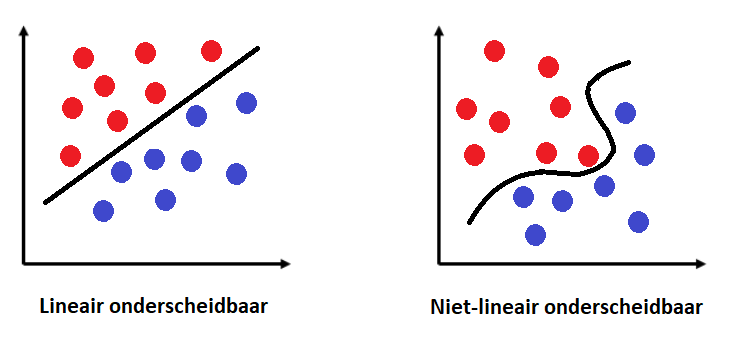
\includegraphics[width=\linewidth]{img/Lineair_onderscheidbaar.png}
	\caption{Lineair onderscheidbaar}
    \label{tab:lineair}
	
\end{figure}


\begin{figure}
	
	
	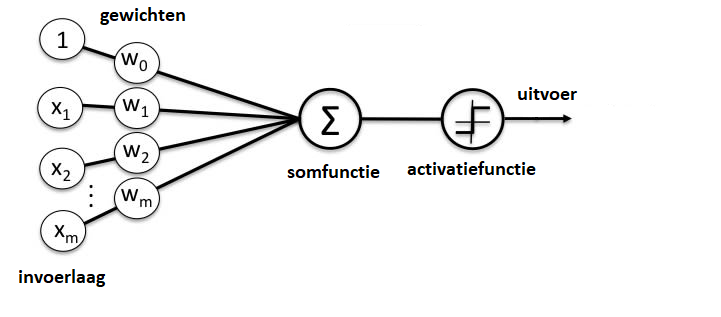
\includegraphics[width=\linewidth]{img/Perceptron.png}
	\caption{Architectuur van een Perceptron}
	\label{tab:perceptron}
\end{figure}

Een meer geavanceerd neuraal netwerk is een netwerk met meerdere lagen, waarbij elke laag een groot aantal neuronen bevat, de eerste laag is altijd de invoerlaag en de laatste laag is altijd de uitvoer laag, de gekende data wordt ingevoerd in de invoerlaag en vervolgens wordt een resultaat berekend dat terug te vinden is in de uitvoerlaag. De daar in tussen liggende lagen worden 'hidden layers' genoemd, hierin krijgen de neuronen een invoer en produceren ze een gepaste uitvoer door middel van een activatie functie.
Elk neuron in een laag is vervolgens verbonden met elk neuron in de daaropvolgende laag waardoor de neuronen genoeg informatie krijgen om te beslissen welke output ze moeten doorgeven naar de volgende laag.

Neurale netwerken kunnen gebruikt worden bij fotoherkenning.
Neem nu een simpel voorbeeld van een artificieel neuraal netwerk dat moet beslissen of een foto een appel of een banaan bevat.
Het netwerk heeft drie verschillende vragen.


\begin{itemize}
	\item Is het voorwerp in de foto rond?
	\item Is het voorwerp in foto geel?
	\item Heeft het voorwerp in de foto een steel?
\end{itemize}

Bij een foto van een banaan zouden de neuronen antwoorden met respectievelijk neen, ja en neen. Voor een appel zou het antwoorden met respectievelijk ja, neen en ja. Met het gebruik van binaire getallen zou het netwerk aanleren dat de output voor een banaan 010 bevat en voor een appel 101.
Wanneer dit voorbeeld wordt uitgeschreven over een groot aantal neuronen lagen is het mogelijk om veel complexere problemen aan te pakken.

deep learning is een redelijk nieuwe term aangezien het pas voor het eerst werd gebruikt rond het jaar 2000. Sindsdien is het een veelgebruikte term en is het een regelmatig besproken onderwerp binnen het vak van artificiële intelligentie. \autocite{Goff2018}


\section{Convolutional Neural Network}

Een 'Convolutional Neural Network', ook bekend onder CNN of ConvNet, is een neuraal netwerk dat zich specialiseert in het verwerken van data dat roostervormig is, zoals een afbeelding. 


Een digitale afbeelding is een binaire representatie van visuele data. Het bevat een reeks van pixels geordend in een rooster waarbij de pixelwaarden aantonen hoe licht en de kleur die de pixel moet weergeven.

Een CNN bestaat, net zoals bij een normaal neuraal netwerk, uit een invoerlaag, een uitvoerlaag en een aantal tussenliggende lagen.
Maar wat een CNN een CNN maakt zijn de tussenliggende lagen waarvan sommige convolutioneel of pooling zijn, de twee belangrijkste lagen in een CNN.

\subsection{Convolutionele laag}




\begin{figure}
	
	
	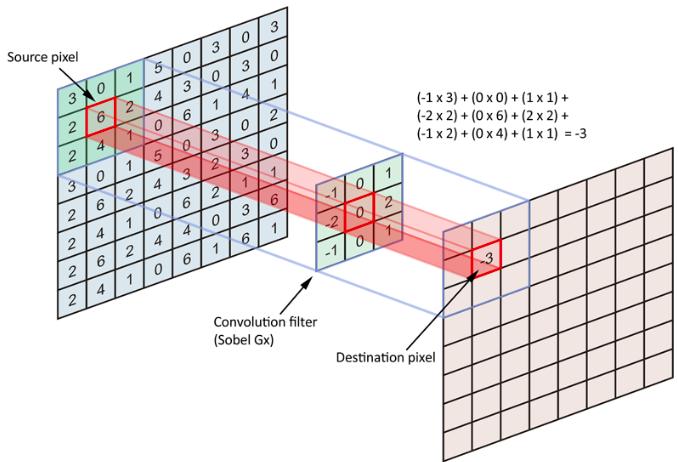
\includegraphics[width=\linewidth]{img/convolution.png}
	\caption{Het convolutional proces}
	\label{tab:convolutional}
\end{figure}

Het verschil tussen een convolutionele laag en een normale laag is dat convolutionele lagen 
lokale patronen in kleine roosters van twee dimensies, details dus, aanleert en een normale laag globale patronen aanleert over het geheel van de afbeelding.

Het grootste doel van een convolutionele laag is om randen, lijnen, vormen, enz. te herkennen.
Vanaf he ogenblik dat het zo een karakteristiek op een specifieke plaats heeft aangeleerd kan het het later in elke andere plaats herkennen. Terwijl een normale laag de karakteristiek opnieuw zou moeten aanleren.

Wanneer een tweede convolutionele laag volgt op een andere convolutionele laag kan de tweede laag aangeleerde patronen gebruiken van de voorgaande laag.
De tweede laag kan daardoor veel geavanceerde patronen aanleren, zoals een oog of een voetbal.

De convolutionele lagen werken met 3 dimensionale roosters, twee assen hiervan tonen de hoogte en breedte aan en de derde de diepte. Wanneer een afbeelding kleuren bevat zal deze diepte 3 lagen bevatten, bij een zwart-wit foto zal deze 1 bevatten.

Een convolutionele laag is convolutioneel aangezien het een convolutionele operatie uitvoert.
Stel nu dat na een invoerlaag een convolutionele laag is geplaatst
dan krijgt de convolutionele laag de niet verwerkte invoer binnen.
De laag maakt een of meerdere vensters aan, die een filter worden genoemd, met meegegeven hoogte en breedte, en per vak krijgt het een willekeurige waarde. Er kan verondersteld worden dat deze filter verschuift over de gehele afbeelding. Voor elke positie dat de filter kan aannemen op de afbeelding is er een verbonden neuron.
Wanneer het venster enkele waarden in de afbeelding opneemt verwerkt hij dit met de willekeurige waarden en de uitvoer wordt in een nieuw rooster geplaatst genaamd een 'feature map', de afbeelding wordt zodanig kleiner.(Figuur \ref{tab:convolutional})

Dit proces wordt duidelijker met een voorbeeld.
Gegeven is een afbeelding van grootte 32x32 (hoogte x breedte),
De afbeelding wordt ingevoerd in de convolutionele laag en deze maakt een filter aan met groote 3x3.
De aangemaakte filter krijgt zijn willekeurige waarden en begint links van boven bij de afbeelding, hier verwerkt de filter de waarden en plaatst ze in een nieuw rooster. 
Vervolgens schuift de filter met een stap naar rechts, wanneer deze filter niet meer naar rechts kan verschuiven, verschuift het met een stap naar beneden en begint opnieuw aan de linkerkant van de afbeelding.
Wanneer de filter op alle unieke posities is geweest is het nieuwe rooster gevormd. Bij dit voorbeeld heeft het nieuwe rooster een grootte van 30x30 aangezien dit het aantal unieke posities is dat de filter kan aannemen.
De convolutionele laag gebruikt voor elk neuron dezelfde filter, een filter kan een enkele karakteristiek herkennen, daarom wordt het aangeraden om meerdere filters te gebruiken in een convolutionele laag.
Wanneer meerdere filters worden gebruikt kunnen meerdere karakteristieken worden herkent en zullen betere resultaten worden opgeleverd.



\subsection{Pooling laag}

Naast de convolutionele lagen zijn ook de pooling lagen belangrijk in het proces van een CNN.
De pooling lagen worden meestal net na een convolutionele laag geplaatst. Een dergelijke laag versimpelt de informatie die verkregen werd door de convolutionele laag door een compactere versie te maken van deze informatie.
Er zijn twee manieren waarop een pooling laag dit kan doen, max-pooling en average-pooling, de meeste gebruikte hiervan is de eerste.

De pooling laag maakt zoals bij een convolutionele laag een filter van meegegeven grootte, vervolgens begint de filter in de hoek links van boven en neemt, bij max-pooling, de grootste waarde in de filter en plaatst deze vervolgens in een nieuw rooster. Wanneer dit is voltooid schuift de filter door naar een volgende positie maar overlapt niet met informatie waar het al is geweest, in tegenstelling tot de filter bij een convolutionele laag.
Bij average-pooling neemt de filter het gemiddelde van de waardes die te zien zijn in de filter.
Stel nu dat de meegegeven hoogte en breedte 2 bevat, dan zal het verwerkte rooster half zo groot zijn als het originele rooster.(Figuur \ref{tab:pooling})\\
Zoals hierboven vermeld heeft een convolutionele laag vaak meerdere filters, wanneer we een pooling laag introduceren in het neuraal netwerk zal het evenveel pooling filters bevatten als convolutionele filters.

\begin{figure}
	
	
	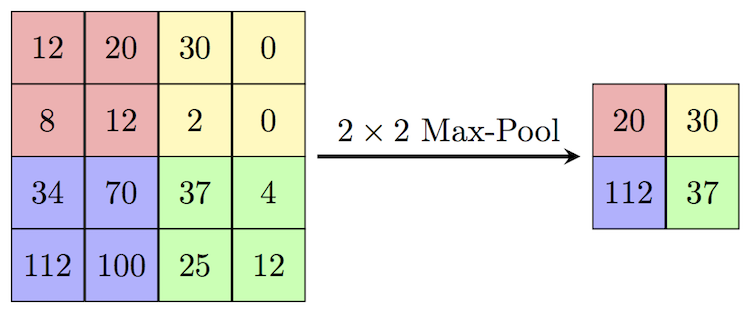
\includegraphics[width=\linewidth]{img/pooling.png}
	\caption{Het max-pooling proces}
	\label{tab:pooling}
\end{figure}

\section{Karakterherkenning}

Een convolutioneel neuraal netwerk kan voor een aantal onderwerpen gebruikt worden zoals, stemherkenning, classificatieproblemen \autocite{Yann1997}, het herkennen van handgeschreven zip code waarden\autocite{J.S.}, enzoverder.
Een onderwerp waarvoor convolutionele neurale netwerken veelal voor gebruikt worden is karakterherkenning of OCR (Optical Character Recognition), een technologie waarbij uit een afbeelding of tekstdocument alle tekens uit het bestand kunnen worden herkend en apart kunnen worden opgeslagen.
Een voorbeeld hiervan is nummerplaatherkenning bij flitspalen. waarbij een foto wordt getrokken, en vervolgens wordt opgeslagen onder de herkende nummerplaat.
Karakterherkenning kan ook te pas komen bij het herkennen van handgeschreven karakters, een probleem dat hierbij voorkomt is dat schriften vaak kunnen variëren in stijl maar dezelfde patronen komen vaak terug.
Dit probleem kan dus opgelost worden met een convolutioneel neuraal netwerk aangezien dit deze vaak terugkomende patronen kan onthouden en simpelweg kan herkennen op andere plaatsen dan de originele gevonden plaats.

Wanneer onderzocht wordt naar karakterherkenning met behulp van een CNN zullen de onderzoekers vaak trachten karakters of woorden te herkennen uit een specifiek schriftsysteem. \autocite{Yoshua}\autocite{Yann}
Even zoeken op het internet en vele artikels kunnen teruggevonden worden die dit specifiek onderzoek toepassen, zoals het herkennen van woorden in het Latijnse schrift \autocite{Aiquan2012}, het herkennen van Chinese karakters \autocite{Weixin}, het herkennen van het Bengaals alfabet, een schriftsysteem uit Zuid-Azië \autocite{Mahbubar2015}, enzovoort.
Deze onderzoeken trachten verschillende karakters uit een gekozen schriftsysteem te herkennen en zodanig woorden te vormen en uiteindelijk deze te lezen. Dit proces is simpelweg het lezen van tekst door middel van een CNN, wat vooral gebruikt kan worden bij het lezen van onbekende schriftsystemen maar veronderstelt dat het gebruikte schriftsysteem al gekend is.

Deze veel voorkomende onderzoeken zijn uitermate interessant aangezien het een beeld geeft van wat mogelijk is en wat niet.
De onderzoeken volgen meestal dezelfde werkwijze, eerst en vooral wordt voldoende data verzameld van het specifieke schriftsysteem. Dit meestal uit al bestaande datasets.
Wanneer men spreekt over datasets zijn er twee groepen te onderscheiden, online datasets en offline datasets.
Bij een online handgeschreven karakter dataset zijn de karakters opgeslagen wanneer de 'gebruikte pen' werd opgeheven en wanneer die werd neergezet, dit kan bijvoorbeeld komen door het gebruik van een smartphone waarbij de 'gebruikte pen' de vinger op het scherm is. \autocite{Cheng-Lin2011}
Een voorbeeld hiervan is de CoMNIST dataset, een dataset bestaande uit het Latijnse schriftsysteem en het Cyrillische. Bij deze dataset kan iedereen participeren met de opslag van de handgeschreven karakters.
De ontwerpers van de dataset maakten een website aan waarbij je een opgegeven letter krijgt, deze letter moet je vervolgens tekenen in een venster en deze wordt opgeslagen in de dataset.
Een offline dataset daarentegen bestaat uit data die gelezen zijn uit documenten of afbeeldingen, deze zijn vaker niet handgeschreven.

Om verder te gaan op de veelgebruikte werkwijze in de al bestaande onderzoeken is de volgende stap het verwerken van de datasets zodanig dat die simpelweg gebruikt kan worden voor de volgende stap.
Hoe een dataset verwerkt wordt hangt af van de technologieën die worden gebruikt en persoonlijke preferentie.
In een bepaald onderzoek wordt de afbeelding geroteerd, verschoven en uitgerekt om zodanig lokale vervorming te creëren, hierdoor komt er meer variëteit in de data. \autocite{Weixin}
Wat vooral voorkomt is het veranderen van de grootte van de data specifiek voor de verwachte invoer van het gebruikte model. \autocite{Aiquan2012} \autocite{Mahbubar2015}
Aan het einde van de nodige aanpassingen van de data volgt er vaak een laatste stap, namelijk de normalisatie van de te gebruiken data.
Normalisatie is het aanpassen van alle data zodanig dat de waarden van alle bijkomende variabelen op een zelfde schaal terecht komen.

De volgende stap is het aanmaken van het model, er wordt gezocht naar de lagen die de beste resultaten op zullen leveren en zorgen dat elke laag de correct invoer krijgt.
Wanneer het model is aangemaakt wordt het getraind met de verwerkte datasets, wanneer dit is gebeurd wordt het model getest en de resultaten worden neergeschreven.

Bij elk onderzoek is zoals verwacht een conclusie uitgeschreven, in de meeste conclusies wordt er uitgelegd dat het gelukt is om een model te schrijven voor hun karakterherkenning.
Maar de inhoud van de conclusies bevatten vaak een redenering dat hun model nog kan worden verbeterd. \autocite{Ahmed2017}
Eén onderzoek blinkt hier wel in uit, dit onderzoek concludeert dat ze een hoge accuraatheid hebben bereikt met hun model. Het verschil met de andere onderzoeken is dat zij niet enkel een CNN gebruiken maar ook andere technologieën gebruiken, dit zijn vooral technologieën die gebruikt worden voor verdere verwerkingen van de gebruikte datasets. \autocite{Yann}

\section{Schriftherkenning}

Rond het kader van karakterherkenning valt veel onderzoek terug te vinden, dit vooral in verband met karakterherkenning van specifieke schriftsystemen.
Een specifieker onderzoeksthema rond het kader van karakterherkenning is het kunnen onderscheiden van verschillende schriftsystemen, dit onderzoeksthema is weinig onderzocht maar kan een groot voordeel bieden aan het onderzoek van karakterherkenning.
Dit vooral wanneer documenten moeten worden ontcijferd die meerdere schriftsystemen bevatten. Een simpel voorbeeld hiervan is de Japanse letterkunde. Deze gebruiken verschillende schriftsystemen. Wanneer deze van elkaar onderscheiden kunnen worden in een document zou het vervolgens eenvoudiger worden om deze te vertalen met een ander karakterherkenningsysteem aangezien het gebruikte schriftsysteem al gekend zou zijn.

Wanneer wordt gekeken naar het al onderzochte in verband met het herkennen van verschillende schriftsystemen is de gebruikte werkwijze gelijkaardig aan de werkwijze dat de onderzoeken gebruiken bij het identificeren van karakters bij een specifiek schriftsysteem.
De data wordt verzameld en verwerkt zodanig dat het kan ingevoerd worden in het aangemaakte model, dat de volgende stap inhoud.
Uiteindelijk wordt het model getest en is een bijhorende conclusie aanwezig.

In de teruggevonden onderzoeken is de conclusie steeds positief, een hoge accuraatheid is bereikt bij de testen maar het model maakt nog enkele fouten bij het onderscheiden van de schriftsystemen. Dit verklaren ze aangezien een aantal schriftsystemen dezelfde karakters delen, wanneer een woord bestaat uit een groot aantal karakters die de twee schriften met elkaar delen is het ingewikkelder voor het model om deze van elkaar te onderscheiden. \autocite{Adman2015}

De gebruikte data bestaat uit afbeeldingen van volledige woorden \autocite{Baoguang2015} of van volledige paragrafen \autocite{Guo2009}.
Dit zorgt ervoor dat het model enkel gebruikt kan worden op volledige woorden of volledige paragrafen. Wanneer men een enkel karakter zal proberen te herkennen zal dit minder accurate resultaten opleveren.
Dit kan wel een oplossing bieden voor het probleem waarbij een aantal karakters worden gedeeld tussen verschillende schriftsystemen.
Wanneer het model wordt getraind op volledige woorden of paragrafen en zo een karakter tegenkomt, die ook voorkomt in andere schriftsystemen, kan het kijken naar de andere karakters die ook voorkomen in het woord of de paragraaf.

Bij een aantal schriften kan het voorvallen dat een groot aantal karakters ook gebruikt wordt door andere schriften.
Een voorbeeld hiervan is het Kanji, het schriftsysteem gebruikt in Japan, en het Hanzi, het schriftsysteem gebruikt in China.
Het Kanji heeft een groot aantal karakters van het Hanzi geadopteerd, vervolgens ondergingen beiden hun eigen evolutie en zijn er momenteel kleine verschillen tussen de twee schriften maar het is nog steeds ingewikkeld om ze van elkaar te onderscheiden. \autocite{Koichi2010}

Onder de terug gevonden artikels gebruikt enkel een hiervan een convolutioneel neuraal netwerk \textcite{Baoguang2015}.
Dit artikel concludeert dat het hoge resultaten behaalt met het gebruik van een CNN.

Onderzoek naar het kunnen herkennen van een alleenstaand karakter is niet teruggevonden, steeds trachten de artikels volledige woorden of paragrafen te herkennen.



















%%=============================================================================
%% Methodologie
%%=============================================================================

\chapter{\IfLanguageName{dutch}{Methodologie}{Methodology}}
\label{ch:methodologie}

%% TODO: Hoe ben je te werk gegaan? Verdeel je onderzoek in grote fasen, en
%% licht in elke fase toe welke stappen je gevolgd hebt. Verantwoord waarom je
%% op deze manier te werk gegaan bent. Je moet kunnen aantonen dat je de best
%% mogelijke manier toegepast hebt om een antwoord te vinden op de
%% onderzoeksvraag.

In dit hoofdstuk zal de gebruikte werkwijze van het onderzoek diepgaand uitgelegd worden met de nodige verantwoording.

Dit onderzoek stelt een werkwijze voor om handgeschreven karakters te classificeren per schriftsysteem aan de hand van een convolutioneel neuraal netwerk.
De gebruikte werkwijze bestaat uit verschillende fasen en die komen in dit hoofdstuk aan bod.


\section{Dataverzameling}

De eerste stap in de werkwijze van dit onderzoek was het nagaan welke datasets nodig waren om het model te trainen.
Het doel van het model is om handgeschreven karakters te classificeren per schriftsysteem, hiervoor waren verschillende datasets van meerdere schriftsystemen nodig, deze bestaande uit de afbeeldingen van handgeschreven karakters.

Een grote factor die invloed had op de keuze van de schriftsystemen lag bij de beschikbaarheid van datasets van het schriftsysteem.
Wanneer een potentieel schriftsysteem werd gekozen moest het toeval er bij liggen dat er een dataset bestond waarbij de data bruikbaar was en uit voldoende data bestond.
Als de dataset niet voldeed aan de eisen werd de dataset achterwege gelaten.
Vervolgens werd er of naar een andere dataset gezocht of werd het schriftsysteem niet gebruikt.



Geweten is dat er 3 grote groepen zijn bij de schriftsystemen, het lag voor de hand om één schriftsysteem te gebruiken per groep.

Het eerste schriftsysteem dat voldeed aan de eisen was het Latijns schrift, dit onder de CoMNIST dataset.
De dataset is een online dataset aangezien de data wordt verzameld door middel van een webapplicatie waar iedereen aan kan deelnemen.
Deze dataset bestaat uit twee mappen, één daarvan is het Latijns schrift, de andere is het Cyrillisch schrift dat in dit onderzoek niet gebruikt zal worden.
Het Latijns schrift wordt vooral gebruikt in de westerse wereld, dit is de reden waarom het een eerste en simpele keuze was.
Dit schrift valt onder de alfabetische groep en vult al één van de drie plaatsen op.

De tweede plaats werd opgevuld door het Kanji, één van de schriften gebruikt in het Japans.
Dit schrift valt onder de logografische groep en is daardoor een goede tweede keuze.
De naam van de dataset is de Kuzushiji-MNIST dataset, een offline dataset.
Deze bestaat uit drie verschillende mappen, enkel de Kuzishiji-Kanji werd gebruikt aangezien dit het grootste aantal aan verschillende karakters bevatte.
Dit zou een voordeel bieden voor het trainen van het model.

Voor de laatste plaats werd er een syllabisch schrift gekozen.
Het gekozen schrift was het Arabisch, een gekend lettergrepenschrift dat vooral in de Arabische wereld wordt gebruikt.
Een dataset in het bezit van \autocite{Ahmed2017}, bestaande uit een groot aantal Arabische karakters.

\section{Datavoorbereiding}

Twee van de drie gekozen datasets zijn bedoeld voor het herkennen van de karakters onder het schriftsysteem van de dataset.
Deze datasets bestonden daardoor uit een structuur van mappen waarbij elke map een specifiek karakter voorstelde uit het schriftsysteem, in elke map zaten vervolgens alle afbeeldingen toebehorend aan dat karakter.

Aangezien in dit onderzoek enkel gezocht werd naar het bijhorende schriftsysteem was het voordelig dat alle afbeeldingen in één grote map zaten.
Er werd hier gesproken over meer dan 10.000 afbeeldingen, deze allen verplaatsen met windows file explorer was geen goede keuze.
Voor deze data verplaatsing werd er eens bash script geschreven dat alles verplaatste. (Tabel \ref{table:BashScript})

\begin{table}[!htbp]
    \begin{tabular}{|l|}
        \hline
        \begin{lstlisting}
find . -mindepth 2 -type f -print -exec mv {} . \;
        \end{lstlisting}
        \\ \hline
    \end{tabular}
    \caption{Bash script voor alle data in één map te verplaatsen. }\label{table:BashScript}
\end{table}

Wanneer al de data voldoende was gestructureerd was het klaar voor de manipulaties die nodig waren voor gebruik.

De datamanipulatie werd gedaan in python, hier waren verschillende libraries voor gebruikt, genaamd numpy, matplotlib, os, tqdm en cv2.
Wanneer een model getraind wordt aan de hand van een groot aantal verschillende afbeeldingen moeten de afbeeldingen allen dezelfde afmetingen bevatten, de keuze voor de hoogte en breedte had invloed op het detailgehalte van de afbeelding, wanneer een lage waarde werd gekozen was er weinig detail te zien, bij een grote waarde was er meer detail te zien.
Voor de afmeting van de afbeeldingen die gebruikt werden bij het model werd een waarde van 60 genomen. (Figuur \ref{tab:afmetingen})


\begin{figure}
    
    
    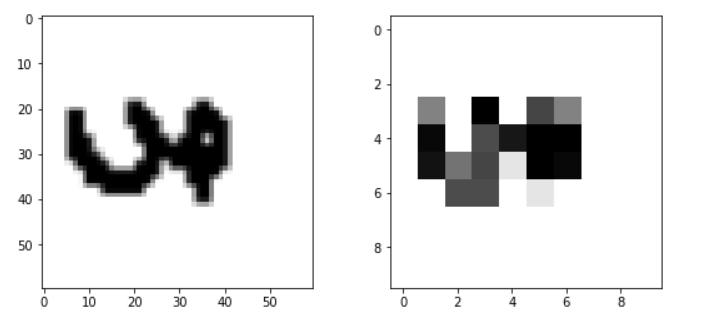
\includegraphics[width=\linewidth]{img/Afmetingen.png}

    \caption{verschil tussen een waarde van 60 (60x60) en een waarde van 10 (10x10) voorgesteld door een Arabisch karakter uit de gebruikte data.}
    \label{tab:afmetingen}
    
\end{figure}

Bij een classificatieprobleem, waar dit onderzoek mee kampt, worden de klassen voorgesteld door numerieke waarden (0, 1, 2, ...). Deze numerieke waarden worden labels genoemd.
Vervolgens worden de afbeeldingen gelinkt aan de bijhorende numerieke waarde.
Bij dit onderzoek zijn de numerieke waarden de schriftsystemen.
Voor het vergemakkelijken voor het model om de data te begrijpen werd er voor gezorgd dat de afbeeldingen allen zwart op wit stonden, de Kanji dataset is bijvoorbeeld wit op zwart dit werd gecorrigeerd.
Als voorlaatste stap werden de afbeeldingen omgezet naar twee-dimensionale matrices waarbij elke waarde in de matrix een waarde voorstelde van de pixel op die positie in de afbeelding.
Uiteindelijk werd de matrix in een lijst geplaatst met de bijhorende label (de numerieke waarde die het schriftsysteem voorstelt). (Tabel \ref{table:DataManipulation})


\begin{table}[!htbp]
    \begin{tabular}{|l|}
        \hline
        \begin{lstlisting}
training_data = []
def create_train_data():
   for category in CATEGORIES: 
      path = os.path.join(DATADIR,category) 
        class_num = CATEGORIES.index(category)
        for img in tqdm(os.listdir(path)): 
          try:
             if(category == "Kanji"):
                 img_array = cv2.imread(
                    os.path.join(path,img),cv2.IMREAD_GRAYSCALE) 
             else:
                 img_array = cv2.bitwise_not(cv2.imread(
                    os.path.join(path,img),cv2.IMREAD_GRAYSCALE))
             new_arr = cv2.resize(img_array,(IMG_SIZE,IMG_SIZE))
             training_data.append([new_arr, class_num])
           except Exception as e:
             pass
        \end{lstlisting}
        \\ \hline
    \end{tabular}
    \caption{Python code voor de manipulatie van de gebruikte datasets (CATEGORIES zijn de gebruikte schriftsystemen) }\label{table:DataManipulation}
\end{table}

De data werd vervolgens willekeurig door elkaar geschud en opgesplitst in twee verschillende lijsten, een lijst van de matrices die de afbeelding voorstelt en een lijst van de bijhorende labels. De positie van een afbeelding in de lijst van matrices ligt op dezelfde positie als de bijhorende label in de andere lijst.
Om de verwerkte data op te slaan werd pickle gebruikt (Tabel \ref{table:DataSave})


\begin{table}[!htbp]
    \begin{tabular}{|l|}
        \hline
        \begin{lstlisting}
import pickle
       
pickle_out = open("X.pickle","wb")
pickle.dump(X, pickle_out)
pickle_out.close()
        \end{lstlisting}
        \\ \hline
    \end{tabular}
    \caption{Het opslaan van de verwerkte data in python door middel van pickle }\label{table:DataSave}
\end{table}

\section{Het Convolutioneel Neuraal Netwerk}

Het ontwerpen van een neuraal netwerk is een proces van trial-and-error.
Een eerste model wordt ontworpen, getraind en als laatste getest, wanneer de accuraatheid van het model niet hoog ligt wordt er gekeken naar het ontwerp van het model.
Er wordt gekeken of er enige aanpassingen nodig zijn voor het verbeteren van de resultaten, wanneer de accuraatheid hoger ligt dan voorheen wordt op dit model verder gewerkt.
Uiteindelijk wordt er een model ontwikkeld dat het best past bij het classificatieprobleem.
In dit hoofdstuk wordt het model besproken dat het best past bij het onderzoek, alsook de verantwoording voor de structuur van het model.

Het model werd ontworpen in python. Voor de implementatie van alle lagen, het laten trainen en testen met de voorbereide data werd tensorflow gebruikt, een open source platform die zich specialiseert in machine learning.
In python werd de library ingeladen zodat de nodige lagen voor een convolutioneel neuraal netwerk gebruikt konden worden.

Aangezien het neuraal netwerk waarden inleest tussen 0 en 1 werden de waarden in de lijst van de lijst van matrices genormaliseerd.
Vervolgens werd de data opgesplitst in traindata waarop het model werd getraind en testdata waarop de accuraatheid van het model werd getest.  \ref{table:DataNormalisition}



\begin{table}[!htbp]
    \begin{tabular}{|l|}
        \hline
        \begin{lstlisting}
X = pickle.load(open("X.pickle","rb"))
y = pickle.load(open("y.pickle","rb"))
       
X = X/255.0

X_train, X_test, y_train, y_test =
       train_test_split(X,y,test_size=0.2)
        \end{lstlisting}
        \\ \hline
    \end{tabular}
    \caption{Het inladen en normaliseren van de data en het opsplitsen van de data} \label{table:DataNormalisition}
\end{table}


Een model wordt aangemaakt en de nodige lagen worden toegevoegd, als eerste laag werd een convolutionele laag geplaatst in het model.
Voor deze laag zijn een aantal parameters nodig, als eerste wordt het aantal filters gevraagd. 
Het aantal filters bepaalt ook het aantal neuronen in de laag, want elke filter is verbonden met een neuron.
De keuze voor het aantal filters ligt bij hoeveel karakteristieken herkend willen worden, aangezien het de eerste laag is werd een aantal van 32 filters gekozen.

Als tweede parameter werd de afmeting gevraagd voor de filter.
De keuze voor de afmeting wordt bepaald door welke soort karakteristieken de filters moeten kunnen verwerken. Wanneer veel detail in de afbeelding aanwezig is zullen kleinere afmetingen worden meegegeven, als grotere karakteristieken moeten herkend worden waar weinig detail aan te pas komt zullen grotere afmetingen worden meegegeven.
Aangezien in de eerste laag vooral simpele karakteristieken zoals vormen, krommingen, et cetera moeten herkend worden werd een afmeting van 5x5 meegegeven.
Als geweten is dat de kleinst mogelijke filter een afmeting van 3x3 bevat zorgt de gekozen afmeting van 5x5 voor het leren van gedetailleerde karakteristieken maar meer rekening houdend met omliggende factoren.

Een derde parameter dat wordt gevraagd is de activatiefunctie, de activatiefunctie bepaalt de uitvoer van de laag.
Voor deze laag werd 'Relu', ook wel 'Rectified linear unit' genoemd, gekozen.

        $f(x) = x^+ = max(0,x)$

Deze functie verandert alle negatieve waarden naar 0 en de positieve waarden blijven hun waarde behouden.
Wanneer deze functie wordt uitgevoerd op een afbeelding blijven enkel de grijze en witte waarden over, de zwarte waarden worden vervangen.
Door deze activatiefunctie wordt het trainingsproces versneld.
(Figuur \ref{tab:Relu})

\begin{figure}
    
    
    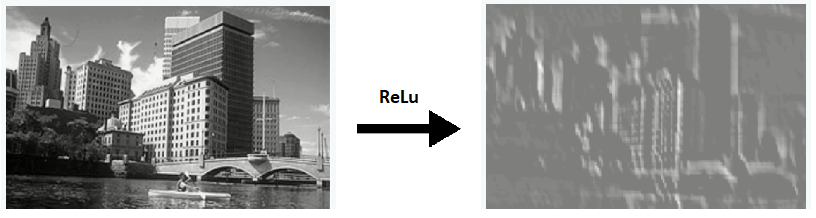
\includegraphics[width=\linewidth]{img/ReLu.png}
    
    \caption{ReLu functie uitgevoerd op een afbeelding.}
    \label{tab:Relu}
    
\end{figure}

Bij de eerste laag in een convolutioneel neuraal netwerk wordt de afmeting gevraagd van de matrices die in de inputlaag zullen worden meegegeven. 

\begin{table}[!htbp]
    \begin{tabular}{|l|}
        \hline
        \begin{lstlisting}
model.add(
    Conv2D(32, (5, 5), activation='relu',input_shape=X.shape[1:]))
model.add(
    MaxPooling2D((2, 2)))

        \end{lstlisting}
        \\ \hline
    \end{tabular}
    \caption{Een eerste convolutioneele laag en een pooling laag}\label{table:FirstLayers}
\end{table}

Nadat een convolutionele laag is toegevoegd aan het model wordt er een pooling laag achter geplaatst.
Bij de pooling laag zijn de verwachte parameters de afmeting van de filters.
Alsook werd deze soort laag toegevoegd aan het neuraal netwerk, 
de gekozen soort pooling laag was een max pooling laag.
Een afmeting van 2x2 werd meegegeven aan de laag.

Een volgende laag dat werd toegevoegd was een convolutionele laag,
een aantal van 64 filters werd gekozen voor deze laag en een afmeting van 7x7.
Het doel van deze laag was het herkennen van grotere patronen met weinig detail, aangezien de vorige laag simpele patronen zou herkennen kon deze laag deze ook gebruiken en zodanig een beter inzicht hebben op de vorm en complexiteit van de karakters.
Net zoals bij de vorige convolutionele laag werd als activatiefunctie ook de Relu functie gekozen.
Vervolgens werd een max-pooling laag toegevoegd met een afmeting van 2x2 voor de filters.

Een derde en laatste convolutionele laag werd nog toegevoegd aan het model met een aantal van 128 filters en een afmeting van 3x3 voor de filters.
Aangezien de afmeting van de filters de kleinst mogelijke waarde bevat staat de laag in voor het herkennen van de details in de karakters.
Deze laag is een belangrijke laag aangezien dit de patronen herkent die eigen zijn aan het schriftsysteem.
Schriftsystemen kunnen onderscheiden worden aan de hand van de kleine details die steeds herkenbaar zijn in de karakters van het schriftsysteem.
Daarom werd een hoog aantal filters meegegeven aan deze laag, zodanig dat de vele details eigen aan de karakters en specifiek aan het schriftsysteem kunnen herkend worden.
Uiteindelijk werd nog een max-pooling laag geplaatst in het model met een afmeting van 2x2 voor de filters.

De convolutionele lagen staan in voor het herkennen van de karakteristieken en patronen, vooraleer een schatting kan verkregen worden van het toebehorende schriftsysteem moeten er nog enkele normale lagen worden toegevoegd.
Er werd gewenst om de uitvoer van de convolutionele lagen in te voeren in normale lagen.
Een convolutioneel neuraal netwerk werkt met invoer in de vorm van 2-dimensionale lijsten.
Een normaal neuraal netwerk daarentegen kan hier niet mee werken, vooraleer de uitvoer van een convolutionele laag in een normale laag kan worden ingevoerd moeten de matrices, 2-dimensionale lijsten, omgevormd worden naar lijsten met 1 dimensie.
Voor deze operatie bestaat er een specifieke laag, de flatten laag.
Na de convolutionele lagen werd zo een dergelijke laag toegevoegd.

Bij een normale laag of dense laag worden ook een aantal parameters gevraagd, waarvan de eerste het aantal neuronen verwacht en de tweede de activatiefunctie verwacht.

Een eerste normale laag werd toegevoegd met een aantal van 128 neuronen en als activatiefunctie werd de ReLu functie gekozen.
Bij deze laag werd een hoog aantal neuronen gekozen aangezien het in staat voor vele karakteristieken en patronen te linken met het toebehorende schriftsysteem.

Een tweede normale laag werd vervolgens toegevoegd aan het model met een aantal van 64 neuronen en als activatiefunctie werd de ReLu functie gekozen.
Deze laag kreeg een normaal aantal neuronen voor de laatste schattingen uit te voeren op de data.

Een probleem dat zich kan vormen in een neuraal netwerk is overfitting,
overfitting is een fenomeen dat zich voor kan doen wanneer een neuraal netwerk zich te veel focust op een specifieke dataset.
Het model zal een goede voorspelling maken op data uit de meegegeven dataset maar wanneer data wordt meegegeven dat het model nog nooit gezien heeft zal het een veel slechtere voorspelling teruggeven.
Om dit probleem tegen te gaan kan een extra laag worden toegevoegd genaamd de dropout laag.
Deze laag doet het volgende, wanneer een model wordt getraind heeft een neuron een kans om gedeactiveerd te worden.
Dit wil zeggen dat het de taak die het neuron op zich heeft niet meer zal uitvoeren.
Dit zorgt voor 'noise', irregulariteit in trainingsproces.
Wanneer een neuron gedeactiveerd wordt neemt een ander neuron de taak op van het inactieve neuron, hierdoor zal het model meer robuuste karakteristieken kunnen aanleren.
Een dropout-laag verwacht een enkele parameter; de kans dat een neuron gedeactiveerd kan worden.
Aan het netwerk werd een dropout-laag toegevoegd met een waarde van 0.1 voor de kans.

De laatste laag van een neuraal netwerk is steeds de uitvoerlaag.
Als uitvoerlaag bij het netwerk werd een normale laag toegevoegd met drie neuronen, een neuron per schriftsysteem.
Voor de activatiefunctie werd de softmax functie gekozen, de softmax functie geeft aan elk neuron een probabiliteit voor elk schriftsysteem.

Wanneer alle lagen waren toegevoegd werd het model gecompileerd en werden nog drie parameters meegegeven.
Een daarvan was de loss functie, dit is de functie die de loss berekend van bij het trainen van een model.
De loss is het aantal fouten die gemaakt worden bij het trainen, het type loss functie die gebruikt wordt hangt af van welk probleem er getracht opgelost te worden met het ontworpen neurale netwerk.
Hier werd als loss functie de 'sparce categorical crossentropy' gekozen, dit aangezien de schriftsystemen verschillende klassen of categorieën voorstellen.\\
Een volgende parameter die gevraagd werd is de optimalisatie functie, deze functie zorgt ervoor dat de gemaakte loss bij een trainingsproces zo laag mogelijk is, dit doet het door de leerbare parameters aan te passen in het neurale netwerk.\\
De laatste parameter die wordt verwacht is de 'metrics', dit zijn waarden die een ontwerper van een model wil dat ze worden weergegeven bij het trainen van het model. ( Tabel \ref{table:Compile})


\begin{table}[!htbp]
    \begin{tabular}{|l|}
        \hline
        \begin{lstlisting}
        model.compile(loss='sparse_categorical_crossentropy',
                      optimizer='adam',
                      metrics=['accuracy'])
        
        \end{lstlisting}
        \\ \hline
    \end{tabular}
    \caption{Het compileren van het model met de nodige instellingen} \label{table:Compile}
\end{table}

\section{Trainen en testen}

Nadat het model gecompileerd was kon er gestart worden met het trainen van het model, hiervoor werd ook tensorflow gebruikt.
Vooraleer het model werd aangemaakt en de nodige lagen waren toegevoegd werd de lijst van data en labels opgesplitst in trainingsdata en trainingslabels en in testdata en testlabels.
Bij het trainen van een model worden de trainingsdata en de trainingslabels meegegeven.
Vervolgens wordt een batch grootte meegegeven die bepaalt hoeveel data het moet testen per keer, het aantal generaties en een splitsing van de data waarbij het opgesplitste deel gebruikt wordt voor validatie.
De validatie zorgt voor een goedkeuring van de data die getraind wordt.
Hier bij het model kreeg de batch grootte een waarde van 32, het werd getraind over 5 generaties en een derde van de data werd gebruikt voor validatie. ( Tabel \ref{table:Training})



\begin{table}[!htbp]
    \begin{tabular}{|l|}
        \hline
        \begin{lstlisting}
       model.fit(X_train, y_train, batch_size=32,
                 epochs=5,validation_split=0.3)
        \end{lstlisting}
        \\ \hline
    \end{tabular}
    \caption{Het trainen van het model met de nodige parameters} \label{table:Training}
\end{table}

\section{Resultaten}

Wanneer het model zijn generaties had voltooid kon gekeken worden naar de accuraatheid en de loss van elke generatie.
De eerste generatie had al een hoge accuraatheid met een waarde van 0.9703 en een lage loss met een waarde van 0.0757.
Bij elke generatie verhoogde de accuraatheid en verlaagde de loss, zoals verwacht.
De laatste generatie had een accuraatheid met een waarde van 0.9993 en een loss met een waarde van 0.0031.
Dit is een hoge accuraatheid en zal zorgen voor een vloeiend onderscheid bij het onderscheiden van de drie schriftsystemen.
Uiteindelijk werd een laatste evaluatie uitgevoerd met de ongeziene testdata en testlabels.
Ook hier was er een hoge accuraatheid van 0.9996 en een lage loss. ( Figuur \ref{tab:testResults})

\begin{figure}
    
    
    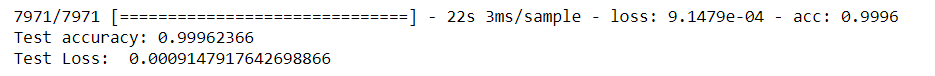
\includegraphics[width=\linewidth]{img/testResults.png}
    
    \caption{Resultaten van de test met weergegeven accuraatheid en loss}
    \label{tab:testResults}
    
\end{figure}

\section{Gebruik}

Een aantal ongekende afbeeldingen werden vervolgens gebruikt met als doel een voorbeeld te geven hoe het gebruikt zou worden in de praktijk.
Een ongekende afbeelding wordt opgeslagen en vervolgens in het model geplaatst.
Eerst en vooral wordt de afbeelding gevormd naar de verwachte afmetingen.
Het model berekent welk schriftsysteem het best past bij de afbeelding en hieruit haalt een script de hoogste waarde uit de lijst van percentages die verkregen zijn vanuit de uitvoerlaag van het model.
Uiteindelijk kijkt het gebruikte script naar de overeenkomende waarde met de lijst van schriftsystemen en geeft dit weer.
De resultaten zijn steeds correct, bij elke afbeelding van een karakter uit een gebruikt schriftsysteem voorspelt het model het juiste schriftsysteem. (Figuur \ref{tab:examples} )

Het gebruik van deze software zou het meest efficiënt zijn met het gebruik van een bijkomende applicatie op een smartphone.
Bij de volgende probleemstelling wordt voorop vastgesteld dat een volledig model is ontwikkeld dat in staat is om een groot aantal veel gebruikte schriftsystemen van elkaar te onderscheiden. \\
Stel nu dat een geleerde in de forensische letterkunde een opdracht krijgt waarbij hij/zij een document dat geschreven is in een ongekend schriftsysteem moet herkennen en lokaliseren. Vooraleer de letterkundige uit eigen ervaring tracht het schriftsysteem te lokaliseren gebruikt hij eerst de mobiele applicatie op zijn smartphone, hij neemt een foto van een karakter in het document en krijgt vervolgens een voorspeld resultaat. \\
Hiervoor moet de software niet volledig accuraat zijn, aangezien het een ongekend schriftsysteem is zal het ook niet veel gebruikt zijn en bestaat de kans dat het niet aangeleerd is aan het model.
Maar een ongekend schriftsysteem dat niet veel gebruikt wordt stamt vaak af van een ander schriftsysteem waarbij de kans wel bestaat dat het aangeleerd is aan het model. \\
Wanneer de mobiele applicatie het schriftsysteem teruggeeft dat veel eigenschappen deelt met het ongekende schriftsysteem, geeft dit al een goede start aan de letterkundige voor het lokaliseren van het ongekende schrift.

Wanneer gewerkt zou worden met volledige woorden of paragrafen bestaande uit karakters uit een schriftsysteem zouden alle karakters herkend kunnen worden en een pluspunt geven aan het door het model voorspelde schriftsysteem.
Als voor alle karakters een voorspelling is gemaakt zou het schriftsysteem met de meeste pluspunten gekozen worden als resultaat.

 
\begin{figure}
    
    
    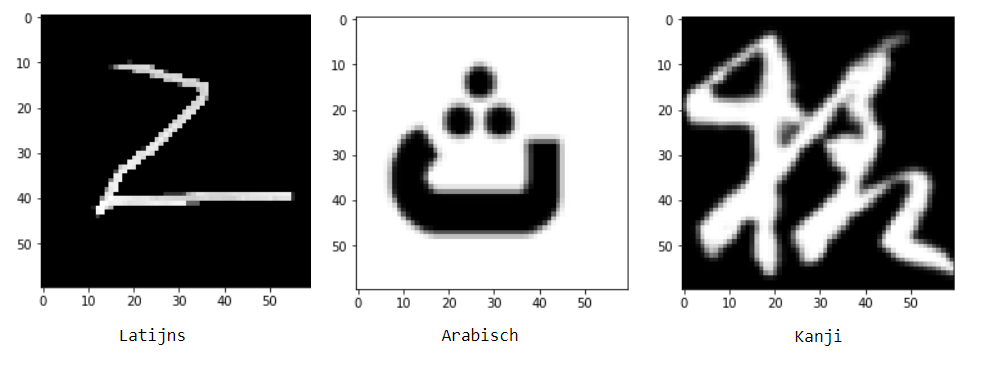
\includegraphics[width=\linewidth]{img/voorbeelden.png}
    \caption{Voorbeelden van het model in de praktijk}
    \label{tab:examples}

\end{figure}









 
















% Voeg hier je eigen hoofdstukken toe die de ``corpus'' van je bachelorproef
% vormen. De structuur en titels hangen af van je eigen onderzoek. Je kan bv.
% elke fase in je onderzoek in een apart hoofdstuk bespreken.

%\input{...}
%\input{...}
%...

%%=============================================================================
%% Conclusie
%%=============================================================================

\chapter{Conclusie}
\label{ch:conclusie}

% TODO: Trek een duidelijke conclusie, in de vorm van een antwoord op de
% onderzoeksvra(a)g(en). Wat was jouw bijdrage aan het onderzoeksdomein en
% hoe biedt dit meerwaarde aan het vakgebied/doelgroep? 
% Reflecteer kritisch over het resultaat. In Engelse teksten wordt deze sectie
% ``Discussion'' genoemd. Had je deze uitkomst verwacht? Zijn er zaken die nog
% niet duidelijk zijn?
% Heeft het onderzoek geleid tot nieuwe vragen die uitnodigen tot verder 
%onderzoek?




%%=============================================================================
%% Bijlagen
%%=============================================================================

\appendix
\renewcommand{\chaptername}{Appendix}

%%---------- Onderzoeksvoorstel -----------------------------------------------


\printbibliography[heading=bibintoc]

\end{document}
